\section{L'esponenziale e la tangente del semiangolo}
\label{sec:semiangolo}

Cinque quaderni --- \texttt{gauss}, \texttt{atan}, \texttt{cosinc},
\texttt{delta} e \texttt{mate} --- contengono pezzi della stessa idea:
scrivere l'esponenziale come funzione razionale della tangente dell'angolo
met\`a. Nessuno la enuncia per intero. Messa insieme, porta a una serie di
risultati classici: la parametrizzazione razionale del cerchio, la funzione
gudermanniana, la frazione continua di Euler per $\ee$, gli approssimanti di
Pad\'e e la trasformazione bilineare dei filtri numerici. Niente di questo
\`e nuovo; vale la pena raccontarlo perch\'e \`e il filo che tiene insieme il
materiale pi\`u interessante della raccolta.

\subsection{Il cerchio e l'asse immaginario}

\begin{prop}\label{prop:semiangolo}
Per $|t|<\pi$, posto $u=\tan(t/2)$,
\begin{equation}\label{eq:cayley}
  \ee^{\ii t}=\frac{1+\ii u}{1-\ii u}=\frac{(1+\ii u)^2}{1+u^2}
  =\sgn(1+\ii u)^2 ,
\end{equation}
dove $\sgn z=z/|z|$. Per ogni $s$ reale, posto $\tau=\tanh(s/2)$,
\begin{equation}\label{eq:tanh}
  \ee^{s}=\frac{1+\tau}{1-\tau},
  \qquad\text{cio\`e}\qquad
  s=\ln\frac{1+\tau}{1-\tau}=2\artanh\tau .
\end{equation}
\end{prop}

\begin{proof}
Poich\'e $\cos(t/2)>0$, si ha $1\pm\ii u=\ee^{\pm\ii t/2}/\cos(t/2)$: il
rapporto vale $\ee^{\ii t}$, e da $1+\ii u=|1+\ii u|\,\ee^{\ii t/2}$ segue
l'ultima forma. Per la seconda parte,
$(1+\tau)/(1-\tau)=(\cosh\frac s2+\sinh\frac s2)/(\cosh\frac s2-\sinh\frac s2)
=\ee^{s/2}/\ee^{-s/2}$.
\end{proof}

Separando parte reale e immaginaria della \eqref{eq:cayley} si ottiene
$\cos t=(1-u^2)/(1+u^2)$ e $\sin t=2u/(1+u^2)$: la parametrizzazione
razionale del cerchio, che per $u=q/p$ razionale d\`a le terne pitagoriche
$(p^2-q^2,\,2pq,\,p^2+q^2)$. Geometricamente $\ee^{\ii t}$ \`e il punto in
cui la retta per $-1$ e per $\ii u$ taglia di nuovo il cerchio: una
proiezione stereografica dal punto $-1$ (figura~\ref{fig:nota_semiangolo},
a sinistra).

La seconda forma della \eqref{eq:cayley} \`e quella che il quaderno scrive in
\righe{gauss.dfw}{1}{4}, osservando anche che $1+u^2$ \`e la derivata di
$2u$ rispetto a $t$: l'esponenziale immaginario come quadrato diviso per una
derivata. La terza forma, con $t$ al posto di $t/2$, compare in
\righe{cosinc.dfw}{1}{3} e in \riga{delta.dfw}{41}.

La \eqref{eq:tanh} \`e la \eqref{eq:cayley} letta sull'asse immaginario:
poich\'e $\tan(\ii y)=\ii\tanh y$, ponendo $t=-\ii s$ si ha
$1\pm\ii u=1\pm\tanh(s/2)$. Il cerchio si apre nella semiretta positiva:
$\tau$ percorre $(-1,1)$ e $\ee^{s}$ percorre $(0,\infty)$. I quaderni
arrivano a questa formula da due lati.

\paragraph{La gaussiana.}
\riga{gauss.dfw}{5} pone $t=\ii x^2$ nella \eqref{eq:cayley} e trova la
gaussiana:
\[
  \ee^{-x^2}=\frac{1-\tanh(x^2/2)}{1+\tanh(x^2/2)} ,
\]
cio\`e la \eqref{eq:tanh} con $s=-x^2$. Il quaderno vorrebbe poi arrivare
alla funzione degli errori integrando $\sgn(1+\ii u)$
(\righe{gauss.dfw}{6}{14}), e la proposizione spiega perch\'e la strada non
porta lontano: sull'asse reale l'informazione sta nella \emph{fase} di
$1+\ii u$, il cui modulo vale $1/\cos(t/2)$; sull'asse immaginario
$1+\ii u=1-\tanh(x^2/2)$ \`e reale e positivo, la sua funzione segno vale
identicamente $1$, e la gaussiana sta tutta nel \emph{modulo}.

\paragraph{L'arcotangente di argomento immaginario.}
\righe{atan.dfw}{1}{14} parte da $\ee^{\ii\arctan x}=(1+\ii x)/\sqrt{1+x^2}$,
che \`e la \eqref{eq:cayley} nella forma $\sgn(1+\ii u)=\ee^{\ii t/2}$, e
sostituisce $x$ con $\ii x$. Per $|x|<1$ vale $\arctan(\ii x)=\ii\artanh x$, e
la riga \#2 trova
\[
  \ee^{\ii\arctan(\ii x)}=\sqrt{\frac{1-x}{1+x}}=\ee^{-\artanh x},
\]
che \`e la \eqref{eq:tanh} con $\tau=x$. Le righe \#3 e \#4 raggiungono il
punto di diramazione $x=1$ ($\arctan\ii=\ii\infty$), e le righe da \#5 a \#14
ricostruiscono la forma logaritmica
$\ii\arctan(\ii x)=\ln(1-x)-\tfrac12\ln(1-x^2)=-\artanh x$, tenendo conto
correttamente dei rami del logaritmo.

\paragraph{La gudermanniana.}
Se lo stesso numero $\tau$ fa da tangente del semiangolo sia per un angolo
circolare $\theta$ sia per un argomento iperbolico $s$, cio\`e se
$\tan(\theta/2)=\tanh(s/2)$, la proposizione d\`a senza passare per i numeri
complessi
\[
  \cos\theta=\frac{1-\tau^2}{1+\tau^2}=\sech s,\qquad
  \sin\theta=\frac{2\tau}{1+\tau^2}=\tanh s,\qquad
  \tan\theta=\frac{2\tau}{1-\tau^2}=\sinh s .
\]
La funzione $s\mapsto\theta=\gd s=2\arctan\bigl(\tanh(s/2)\bigr)$ \`e la
gudermanniana. Le righe \righe{mate.dfw}{111}{122} cercano, per ciascuna
funzione iperbolica, una funzione circolare con lo stesso valore:
$\tanh x=\tan(kx)$, $\sinh x=\sin(kx)$ e cos\`i via. Le risposte di Derive
sono corrette caso per caso --- per esempio $kx=\arctan(\tanh x)$, che vale
$\tfrac12\gd(2x)$ --- ma la risposta sistematica \`e la gudermanniana:
$\tan(\gd x)=\sinh x$, $\sin(\gd x)=\tanh x$, $\cos(\gd x)=\sech x$.

\begin{figure}[t]
  \centering
  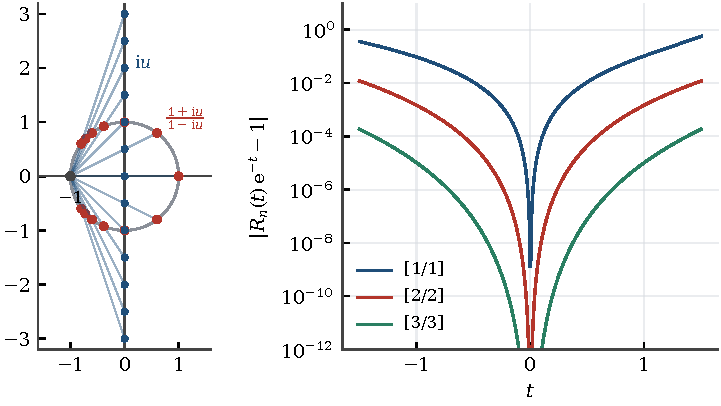
\includegraphics[width=\linewidth]{nota_semiangolo}
  \caption{A sinistra, la proiezione stereografica dal punto $-1$: la retta
  per $-1$ e per $\ii u$ taglia il cerchio in $(1+\ii u)/(1-\ii u)=\ee^{\ii t}$,
  per $u=-3,-2{,}5,\dots,3$. A destra, l'errore relativo degli approssimanti
  di Pad\'e diagonali $R_1$, $R_2$, $R_3$ di $\ee^{t}$, ottenuti troncando la
  frazione continua di Lambert.}
  \label{fig:nota_semiangolo}
\end{figure}

\subsection{Il numero \texorpdfstring{$\ee$}{e} e le frazioni continue}

Con $s=1$ la \eqref{eq:tanh} d\`a
\[
  \ee=\frac{1+\tanh\frac12}{1-\tanh\frac12},
  \qquad
  \tanh\tfrac12=\frac{\ee-1}{\ee+1}=0{,}46211715\dots
\]
Questo numero ha una frazione continua celebre, trovata da Euler nel
1737~\cite{eulero1744}:
\[
  \frac{\ee-1}{\ee+1}
  =\cfrac{1}{2+\cfrac{1}{6+\cfrac{1}{10+\cfrac{1}{14+\dotsb}}}}
  =[0;\,2,6,10,14,\dots],
\]
con i quozienti parziali in progressione aritmetica. Pi\`u in generale, per
ogni intero positivo $n$,
\[
  \tanh\frac1n=[0;\,n,3n,5n,\dots].
\]
Entrambe discendono dalla frazione continua di Lambert~\cite{lambert1768}
\[
  \tanh x=\cfrac{x}{1+\cfrac{x^2}{3+\cfrac{x^2}{5+\dotsb}}} ,
\]
ponendo $x=1/n$ e liberando i denominatori. Lambert la us\`o per dimostrare
che $\tanh x$, e quindi $\ee^{2x}=(1+\tanh x)/(1-\tanh x)$, \`e irrazionale
per ogni $x$ razionale non nullo; la frazione analoga per $\tan x$, con
$\tan(\pi/4)=1$, d\`a l'irrazionalit\`a di $\pi$. Per $\ee$, dunque, la
formula $\ee^{s}=(1+\tau)/(1-\tau)$ \`e proprio un passaggio della prima
dimostrazione di irrazionalit\`a; per $\pi$ ne serve la versione circolare,
con $\tan$ al posto di $\tanh$. I quaderni non arrivano fin qui, ma \`e l\`i
che la loro idea conduce.

\subsection{Troncare: gli approssimanti di Pad\'e}

Troncando la frazione di Lambert per $\tanh(t/2)$ e sostituendo nella
\eqref{eq:tanh} si ottiene, al primo, al secondo e al terzo livello,
\[
  R_1(t)=\frac{2+t}{2-t},\qquad
  R_2(t)=\frac{12+6t+t^2}{12-6t+t^2},\qquad
  R_3(t)=\frac{120+60t+12t^2+t^3}{120-60t+12t^2-t^3}.
\]
Sono gli approssimanti di Pad\'e diagonali $[n/n]$ di $\ee^{t}$: le funzioni
razionali con numeratore e denominatore di grado $n$ che coincidono con
$\ee^{t}$ fino all'ordine $t^{2n}$; per esempio
$R_1(t)-\ee^{t}=t^3/12+O(t^4)$. Che i convergenti della frazione di Lambert
diano esattamente la diagonale della tavola di Pad\'e dell'esponenziale \`e
un fatto generale~\cite{baker1996}; qui lo abbiamo verificato per
$n\le3$. Dalla formula esatta gli approssimanti ereditano due propriet\`a:
$R_n(-t)=1/R_n(t)$, come $\ee^{t}$, e $|R_n(\ii\omega)|=1$ per ogni $\omega$
reale, perch\'e numeratore e denominatore sono coniugati sull'asse
immaginario. Mandano cio\`e l'asse immaginario sul cerchio unitario,
esattamente come $\ee^{\ii\omega}$; anzi $R_1(\ii\omega)$ \`e la
\eqref{eq:cayley} con $u=\omega/2$. L'errore relativo dei primi tre
approssimanti \`e nella figura~\ref{fig:nota_semiangolo}, a destra.

\subsection{Un'applicazione: i filtri numerici}

Un filtro analogico con funzione di trasferimento $H(s)$ si trasforma in un
filtro numerico, con passo di campionamento $T$, esprimendo $s$ attraverso
$z=\ee^{sT}$. Per la \eqref{eq:tanh} la relazione esatta \`e
\[
  \frac{z-1}{z+1}=\tanh\frac{sT}{2},
  \qquad\text{cio\`e}\qquad
  s=\frac2T\artanh\frac{z-1}{z+1},
\]
che non \`e razionale in $z$. La trasformazione bilineare (di Tustin)
sostituisce $\tanh(sT/2)$ con la sua prima approssimazione $sT/2$:
\[
  s\;\mapsto\;\frac2T\,\frac{z-1}{z+1},
  \qquad\text{cio\`e}\qquad
  z=\frac{1+sT/2}{1-sT/2}=R_1(sT).
\]
Poich\'e $|R_1(\ii\Omega T)|=1$ e $|R_1(s)|<1$ per $\Real s<0$, l'asse
immaginario va sul cerchio unitario e il semipiano sinistro nel disco: un
filtro stabile resta stabile. Il prezzo si paga in frequenza: sul cerchio
$z=\ee^{\ii\omega T}$, e la \eqref{eq:cayley} d\`a
$(z-1)/(z+1)=\ii\tan(\omega T/2)$, quindi alla frequenza numerica $\omega$
corrisponde la frequenza analogica
\[
  \Omega=\frac2T\tan\frac{\omega T}{2}.
\]
\`E la distorsione delle frequenze della trasformazione bilineare; il rimedio
abituale, \emph{precompensare} le frequenze critiche con questa stessa
formula, si trova nei manuali di elaborazione numerica dei
segnali~\cite{oppenheim2010}. Se il filtro elimina-banda progettato in
\texttt{notch.dfw} venisse realizzato in forma numerica, la sua pulsazione di
antirisonanza andrebbe precompensata proprio cos\`i: la tangente del
semiangolo di \texttt{gauss.dfw} \`e la stessa dell'ingegnere.

Lo stesso schema compare in relativit\`a ristretta: se $\beta=\tanh\eta$ \`e
la velocit\`a in unit\`a di $c$ e $\eta$ la rapidit\`a, il fattore Doppler
\`e $\ee^{\eta}=\sqrt{(1+\beta)/(1-\beta)}=(1+\tanh\frac\eta2)/(1-\tanh\frac\eta2)$.

\paragraph{Che cosa resta aperto.}
Nulla, sul piano matematico: tutto ci\`o che compare in questa sezione \`e
classico. Quello che i quaderni aggiungono \`e l'aver percorso, senza saperlo,
un tratto della stessa strada da cinque lati diversi.
